\documentclass[11pt]{article}
\usepackage[a4paper, hmargin={2.8cm, 2.8cm}, vmargin={2.5cm, 2.5cm}]{geometry}
\usepackage{eso-pic} % \AddToShipoutPicture
\usepackage{graphicx} % \includegraphics
\usepackage{tabto}
\usepackage{enumerate}
\usepackage{txfonts}
\usepackage{graphicx}
\usepackage{float}

%% Change `ku-farve` to `nat-farve` to use SCIENCE's old colors or
%% `natbio-farve` to use SCIENCE's new colors and logo.
\def \ColourPDF {include/ku-farve}

%% Change `ku-en` to `nat-en` to use the `Faculty of Science` header
\def \TitlePDF   {include/ku-en}  % University of Copenhagen

\title{
  \vspace{3cm}
  \Huge{Some Title} \\
  \Large{More elaborate subtitle}
}

\author{
  \Large{Bjarke Kingo Iversen}
  \\ \texttt{bjarkekingo50@gmail.com} \\\\
  \Large{Susanne Truong}
  \\ \texttt{suzze-t@hotmail.com}
}

\date{
    \today
}

\begin{document}

\AddToShipoutPicture*{\put(0,0){\includegraphics*[viewport=0 0 700 600]{\ColourPDF}}}
\AddToShipoutPicture*{\put(0,602){\includegraphics*[viewport=0 600 700 1600]{\ColourPDF}}}

\AddToShipoutPicture*{\put(0,0){\includegraphics*{\TitlePDF}}}

\clearpage\maketitle
\thispagestyle{empty}

\newpage

%% Write your dissertation here.
\section{Abstract}
\newpage
\tableofcontents
\newpage
%%%%%%%%%%%%%%%%%%%%%%%%%%%%% Introduction %%%%%%%%%%%%%%%%%%%%%%%%%%%%%
\section{Introduction}
It is widely known that it can be time-consuming to choose the wrong path, if you want to travel from one city to another. It will most certainly be faster to aboard the train from Chicago to Seattle, rather than going through Los Angeles before heading to Seattle. Choosing the right path will therefore save a lot of time.\\
The problem herein is that its in lots of cases is nowhere intuitive which path that guarantees the consumation of time to be minimal. We probably can't withstand the big amounts of information if we should compute the shortest path, through millions of combinations by ourselves. For computersystems to choose such a path, they'd need a method for calculating such, an algorithm.\\
Different shortest-path algorithms are known to solve such problems theoretically. We'll examine the theory behind these, and analyse the complexity to see whether the time-complexity given by Bellmann-Ford and Dijkstras algorithms holds in real life implementations, by implementing them with both a binary and a fibonacci-heap in C++, thus finally to match them all up against each other.\\
We'll as well analyse and implement the A*-algorithm to see how well dijkstra match up against this on euclidean planar graphs. Since we're primarily interested in road-maps, we won't consider negative weights.\\

\section{Problem definition}
To examine and benchmark the complexity of different shortest-path algorithms, e.g. Dijkstra, Bellmann-Ford, and A* Search. We will do this by implementing and comparing them using different data structures and libraries. Finally we will compare the results of these experiments with the theoretical bounds.

%%%%%%%%%%%%%%%%%%%%%%%%%%%%%%% Notation %%%%%%%%%%%%%%%%%%%%%%%%%%%%%%%
\section{Notation}
A short list of notations used throughout the thesis:
\begin{itemize}
\item $G(V,E)$ = Graph, consisting of set of vertices V, and set of edges E
\item $s$ = Designated to be the source vertex s
\item $w(u,v)$ = Weighted distance from vertix u to v
\item $d[v]$ = The weigth of the current shortest path from s to v. $d[v]$ is initlized to be $\infty$ for all vertices besides the source vertex. $d[s]$ is initialized to be 0.
\item $\pi[v]$ = Predecessor/parent vertex to v in the current shortest path. $\pi[v]$ is initialized to be NIL. This is set to a vertex once/if a path is discovered from s to v.
\item $\delta(u,v)$ = the weigth of the shortest path from u to v.
\end{itemize}

%%%%%%%%%%%%%%%%%%%%%%%%%%% Shortest Paths %%%%%%%%%%%%%%%%%%%%%%%%%%%
\section{On Shortest Paths}
In the shortest path problem, a graph $G = (V,E)$ is given, where $V$	
is the set of vertices, and $E$ is the set of edges. Each edge
connects two vertices and contains a weight, indicating the cost of
moving between these vertices. By using a shortest path algorithm, we
can find a shortest path $P = {v_{1}, v_{2}, ..., v_{k}} \in V$ from a
given source vertex $s \in V$ to all other vertices $v \in V$. I.e.,
we want to find a path, where the total weight of the visited edges is
minimal.\\

%%%%%%%%%%%%%%%%%%%%%%%%%%%%% Relaxation %%%%%%%%%%%%%%%%%%%%%%%%%%%%%
\noindent
\textbf{Relaxation}\\
When searching for the shortest path from a source vertex $s$ to a
vertex $v$, a shortest-path estimate $d[v]$ is preserved for each
vertex $v \in V$. At first, $d[v]$ will be an overestimate, but if we see that the shortest path to $v$ can be improved by going through a vertex $u$, we update the estimate $d[v]$ with the new and lower cost. As better paths are found, we will eventually get the correct estimate and find the shortest path, if it exists. This technique is called relaxation and is used by the three algorithms that we will talk about later. The pseudocode for relaxing an edge $(u,v) $ is shown below:\footnote{Introduction to Algorithms, pg. 649}\\

%\noindent
\textbf{RELAX$(u, v, w)$}
\begin{enumerate}
\NumTabs{24}
\setlength\itemsep{0em}
\item \textbf{if } $d[v] > d[u] + w(u,v)$
\item \tab{$d[v] = d[u] + w(u,v)$}
\item \tab{$\pi[v] = u$}
\end{enumerate}
(TODO: Explain the pseudocode )\\

\noindent
(Dry run relaxation of an edge? One in which a shortest- path estimate decreases and one in which no estimate changes... -> see pg. 649)\\

%%%%%%%%%%%%%%%%%%%%%%%%%%%%% Properties %%%%%%%%%%%%%%%%%%%%%%%%%%%%%
\section{Proving the correctness of shortest path algorithms}
The shortest path algorithms that we have talked about will always find a shortest path, if it exists. This can be proved by looking at the properties that shortest paths and relaxation have:\footnote{Introduction to Algorithms, pg. 650}

\begin{itemize}
\item \textbf{Triangle inequality}\\
The triangle inequality lemma is a geometric property of triangles which states that the sum of two lengths of any two sides must be greater than or equal to the remaining side. That is, for any triangle with sides $\{x,y,z\}$, we have that $z \leq x+y$.\\\\
Applied to the shortest path problem we have that for any edge $(u,v) \in E$, we have $\delta(s,v)\leq \delta(s,u) + w(u,v)$ (\textbf{Lemma 1}). Thus the shortest path from s to v must be less than or equal to the shortest path from s to u added to the weigth from u to v.\\
\item \textbf{Upper-bound property}\\
The upper-bound property says that our estimate for the shortest distance to v is always greater than or equal to the actual shortest path from s to v, for all vertices v$\in$ V.\\\\
That is $\forall v \in V.(d[v]\geq \delta(s,v))$. Once our estimate holds the actual value for the shortest path, the estimate never changes (\textbf{Lemma 2}).\\
\item \textbf{No-path property (\textbf{Corollary to Lemma 2})}\\
If there is no path from s to v, then we always have $d[v] = \delta(s,v) = \infty$.\\
\item \textbf{Convergence property}\\
The convergence property ensures us that if we from s, at sometime has u to v is the shortest path in G for some u,v $\in$ V, and if the estimated shortest path to u actually is the shortest path, we'd then have (prior to relaxing the edge (u,v)) that the estimated shortest path to v must be the shortest path to v at all times afterward.\\\\
That is, if $s\rightsquigarrow u\rightarrow v$ is a shortest path, and if $d[u] = \delta(s,u)$, then $d[v] = \delta(s,v)$ is assured at all time afterward (\textbf{Lemma 3}).\\
\item \textbf{Path-relaxation property}\\
Our path-relaxation property ensures that the relaxation of a shortest path p will derive that the distance to the k'th vertix in p is equal to the shortest path to vertix k.\\\\
Let $p = \{v_{1}, v_{2},\cdots ,v_{k}\}$ be a shortest path that goes from $v_{1}$ to $v_{k}$. If the edges are relaxed in the order $(v_{1},v_{2}), (v_{2},v_{3}), \cdots , (v_{k-1}, v_{k})$, then $d[v_{k}] = \delta(s,v_{k})$ once the whole path is relaxed \footnote{Shortest Paths: 6.006 Intro to Algorithms, March 30 2011, Recitation 14. MIT}(\textbf{Lemma 4}).\\
\item \textbf{Predecessor-subgraph property}\\
The predecessor-subgraph/parent-subgraph property ensures that once the shortest path to v is computed for all vertices v, the predecessor subgraph is a shorted-paths tree rooted at s.\\\\
Such that once $\forall v \in V.(d[v] = \delta(s,v))$ the predecessor subgraph that contains all the vertices with a finite distance from s, but with only edges that connects v to $\pi[v]$ is a shortest-path tree\footnote{Shortest Paths: 6.006 Intro to Algorithms, March 30 2011, Recitation 14. MIT} (\textbf{Lemma 5}).
\end{itemize}

%%%%%%%%%%%%%%%%%%%%%%%%%%%%% Bellman-Ford %%%%%%%%%%%%%%%%%%%%%%%%%%%%%
\section{Bellmann-Ford algorithm}
...\\
If there is a negative cycle, the cost of the shortest path is decreased every time the algorithm runs through the negative cycle. By doing this numerous times, we can receive arbitrarily negative weights, thus making the cost undefined.\\

See: http://stackoverflow.com/questions/20123076/can-dijkstras-single-source-shortest-path-algorithm-dectect-an-infinite-cycle-i\\


%%%%%%%%%%%%%%%%%%%%%%%%%%%%%%%% Heaps %%%%%%%%%%%%%%%%%%%%%%%%%%%%%%%%%
\section{Min heaps}
In the following section, we will describe min heaps that Dijkstra's algorithm takes in use...\\
DER SKAL FORKLARES OM HOBS OG SÅDAN NOGET!

%%%%%%%%%%%%%%%%%%%%%%%%%%%%%%% Dijkstra %%%%%%%%%%%%%%%%%%%%%%%%%%%%%%%
\section{Dijkstra's algorithm}
Dijkstra's algorithm takes a weighted graph $G = (V, E)$ and finds the shortest path from a single source to each other vertex in the graph. To keep track of the vertices, the algorithm maintains two sets of vertices. The set $S$ consists of vertices, where the optimal shortest-path estimate from the source $s$ has been figured. The other set $Q$ is a minimum priority queue that contains the remaining vertices, i.e. $Q = V - S$. The algorithm will repeatedly extract a vertex with the minimum shortest-path estimate from $Q$ and add it to $S$, until all vertices have been discovered.\\

\noindent 
\textbf{Assumptions}\\
For Dijkstra's algorithm to work, we must assume that the graph contains no negative weights. Once a vertex has been extracted from the min-priority queue, Dijkstra's algorithm will assume that the shortest path to that vertex has been found. This means the algorithm will never have to relax this vertex again. However, if there is a negative-weighted edge somewhere, the algorithm may find a wrong shortest-path.\footnote{http://stackoverflow.com/questions/13159337/why-doesnt-dijkstras-algorithm-work-for-negative-weight-edges} An example can be seen in the following figure:\\

\begin{figure}[H]
\centering
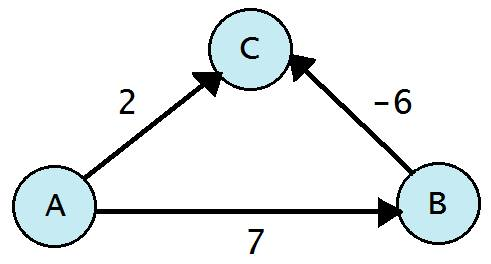
\includegraphics[scale=0.3]{neg-weight.png}
\caption{A graph with negative weights}
\end{figure}

\noindent In this figure, the graph consists of three vertices $A, B,$ and $C$. Dijkstra's algorithm starts at the source $A$ and will first extract $C$, since it has the shortest-path estimate of 2. Afterwards, the algorithm extracts the last vertex $B$ and terminates. Had it however tried to relax the negative edge between $B$ and $C$, a shorter path of $7 - 6 = 1$ would have been discovered. The result is therefore incorrect due to dijkstra utilizing the greedy property of \textbf{Lemma 1}, thus that $\forall (u,v) \in E.(w(u,v) \geq 0)$. \\

\noindent
(\textbf{Does the graph have to be connected???}\\
A connected graph means that for all $v \in V $,a vertex $v$ will be reachable from another vertex $w$ through an edge. If the graph is disconnected, some vertices will be unreachable, thus making some shortest paths infinite, if we try to reach these vertices.)\\\\


\noindent
\textbf{How Dijkstra's algorithm work}:\\
The pseudocode for Dijkstra's algorithm can be seen below:\footnote{Introduction to Algorithms, pg. 658}\\

\textbf{DIJKSTRA$(G, w, s)$}
\begin{enumerate}
\NumTabs{24}
\setlength\itemsep{0em}
\item INITIALIZE-SINGLE-SOURCE$(G, s)$
\item $S = $ \O
\item $Q = G.V$
\item $\textbf{while } Q \neq$ \O
\item \tab{$u = $ EXTRACT-MIN$(Q)$}
\item \tab{$S = S \cup \{u\}$}
\item \tab{\textbf{for} each vertex $v \in G.Adj[u]$}
\item \tab{}\tab{RELAX$(u,v,w)$}
\end{enumerate}

\noindent (TO DO: explain the pseudocode and dry run an example)\\








%%%%%%%%%%%%%%%%%%%%%%%%% Dijkstra  modified %%%%%%%%%%%%%%%%%%%%%%%%%
\noindent The original pseudocode finds the shortest path from a source vertex to all other vertices. We are only interested in finding the shortest path for a single target. so we have modified the original pseudocode for Dijkstra's algorithm. As soon as the algorithm finds the shortest path to the target vertex, it will terminate. This will reduce the amount of vertices visited, unless the target happens to be the last vertex found.\\

\textbf{MODIFIED-DIJKSTRA$(G, w, s, t)$}
\begin{enumerate}
\NumTabs{24}
\setlength\itemsep{0em}
\item $d[s] = 0$
\item $S = Q = \{s\}$
\item $\textbf{while } Q \neq  $ \O
\item \tab{$u = $ EXTRACT-MIN$(Q)$}
\item \tab{\textbf{if } $u = t$}
\item \tab{}\tab{\textbf{Terminate}}
\item \tab{\textbf{for} each vertex $v \in G.Adj[u]$}
\item \tab{}\tab{\textbf{if } $v \notin S$}
\item \tab{}\tab{}\tab{$S = S \cup \{v\}$}
\item \tab{}\tab{}\tab{$Q = Q \cup \{v\}$}
\item \tab{}\tab{}\tab{$d[v]  = d[u] + w(u,v)$}
\item \tab{}\tab{}\tab{$\pi[v] = u$}
\end{enumerate}

\noindent The pseudocode now takes a 4th parameter $t$, indicating the target vertex we want to find. Instead of calling the function \textit{INITIALIZE-SINGLE-SOURCE}, we only set the source's shortest-path estimate to 0. All other vertices are already assumed to have a shortest-path estimate equal to $\infty$, so it is not necessary to initialize the estimates to $\infty$.\\
The set $S$ still contains the set of vertices whose optimal shortest-path estimates have been determined. At start, only the final estimate is known for the source vertex $s$ (line 2). The min-priority queue Q has also been modified to contain $\{s\}$, since we only want to insert new vertices into the queue, as they are discovered. Line 4 extracts a vertex $u$ with the minimum shortest-path estimate. If the vertex $u$ is the target vertex, the algorithm terminates. Else, the algorithm examines each vertex $v$ that is adjacent to $u$ in line 7. If $v$ has not been examined before, it will not be an element of $S$, since the shortest-path estimate is still $\infty$ and need to be relaxed...




linje 9-12...
From the properties of Dijkstra's, we have that $d[u] = \delta(s,u)$. 
From the convergence property... something with adding w(u,v) will give the optimal d[v]. 

To move onwards from vertex $v$, the vertex must also be inserted into the min-priority queue $Q$ in line 10.




\noindent Figure 1 illustrates the difference between the two algorithms.\\
\begin{figure}
\centering
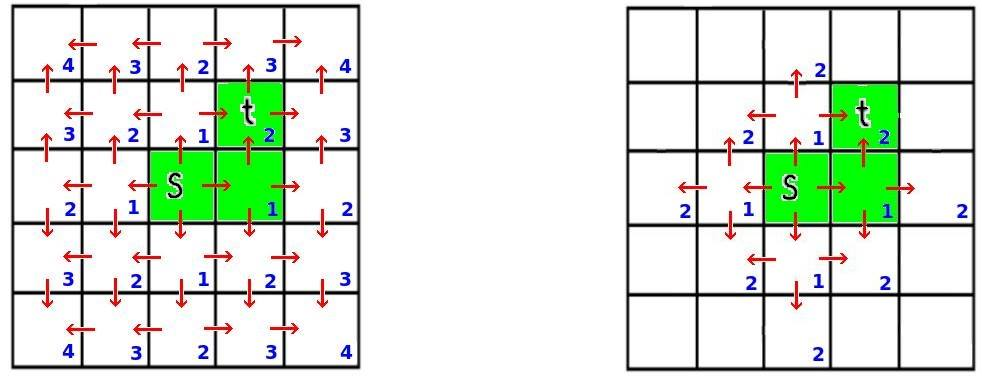
\includegraphics[scale=0.5]{dijkstra.png}
\caption{Dijkstra's algorithm vs. the modified Dijkstra's algorithm}
\end{figure}




%%%%%%%%%%%%%%%%%%%%%%%%%%%%%%% A* search %%%%%%%%%%%%%%%%%%%%%%%%%%%%%%%
\section{A* search}
...\\



\section{Results}
\section{Bibliography}

\end{document}
